%
% ─── CAPITULO 3: CONJUNTOS DE JULIA Y MANDELBROT ────────────────────────────────
%

Terminamos el capítulo \ref{chap:iteracion} fijándonos en la autosimilaridad de las imágenes que nos proporcionaba la aplicación del método de Newton en ciertas funciones complejas para deducir las cuencas de atracción de las distintas funciones. Pudimos comprobar que a pesar de ser imágenes que no son totalmente autosimilares, por lo que no son fractales en el sentido estricto, contienen fragmentos que sí lo son. Este mismo hecho se produce en los conjuntos de Julia y en el conjunto de Mandelbrot. Podemos observar este hecho en las imágenes \ref{fig:julia-intro}, que son nuestros primeros dos ejemplos de conjuntos de Julia.

\begin{figure}[ht]
    \centering
    \begin{tabular}{cc}
      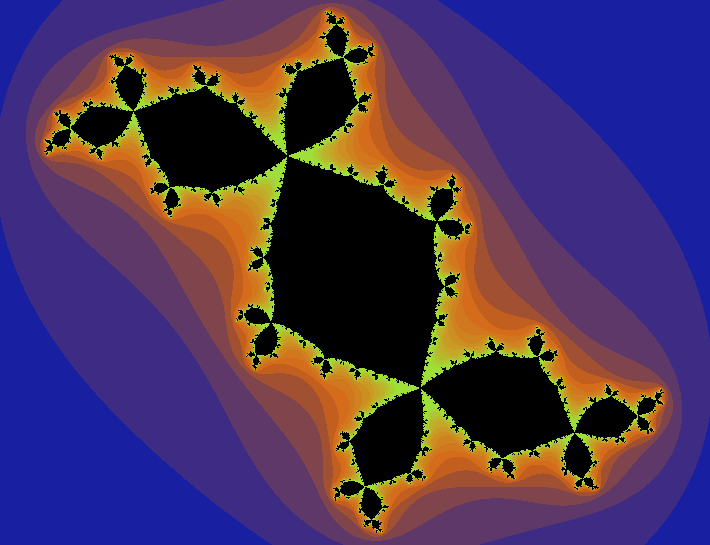
\includegraphics[scale=0.28]{./img/C3/julia-intro-2.png} &   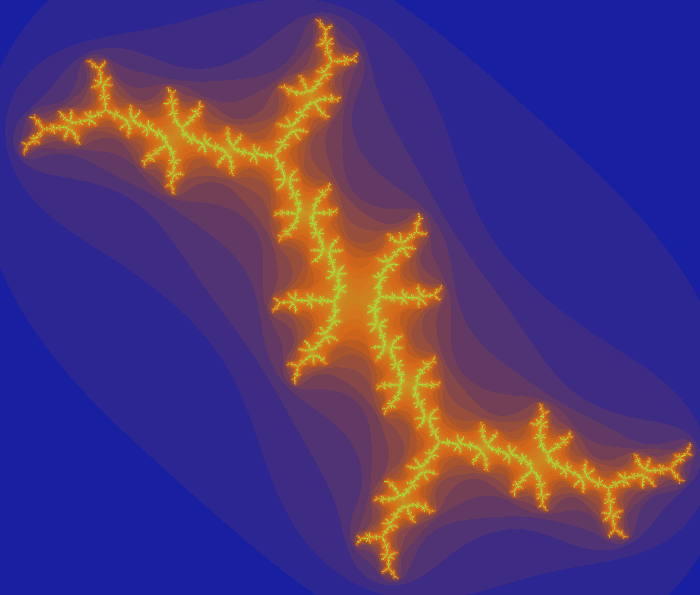
\includegraphics[scale=0.255]{./img/C3/julia-intro-1.png} \\
    (a) Conjunto de Julia conexo & (b) Conjunto de Julia no conexo  \\[6pt]
    \end{tabular}
    \caption{Primeras imágenes de conjuntos de Julia}
    \label{fig:julia-intro}
\end{figure}

Una notable diferencia entre las imágenes \ref{fig:julia-intro} se encuentra en que mientras en la imagen (a) se puede percibir cierta conexión en el conjunto, esta desaparece en el caso de la imagen (b). Precisamente en esa distinción reside la génesis del conocido \textit{conjunto de Mandelbrot}, que podemos también ver por primera vez, junto con algunas de sus autosimilaridades, en las imágenes \ref{fig:mandelbrot-intro}.

\begin{figure}[ht]
  \centering
  \begin{tabular}{cc}
    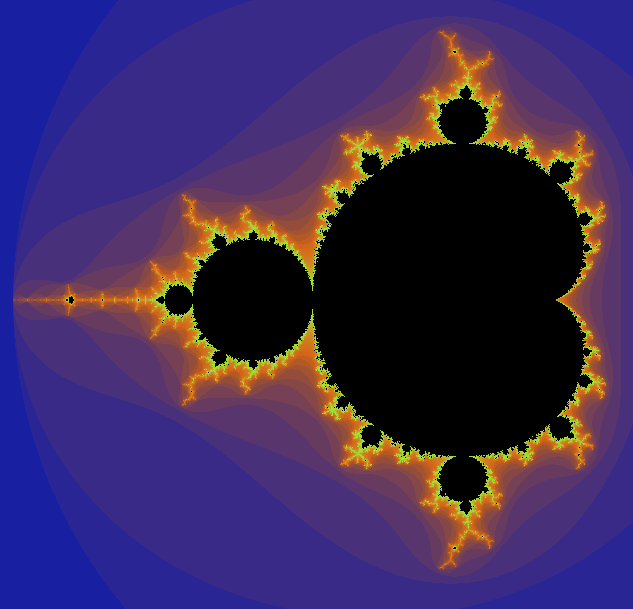
\includegraphics[scale=0.28]{./img/C3/mandelbrot-intro.png} &   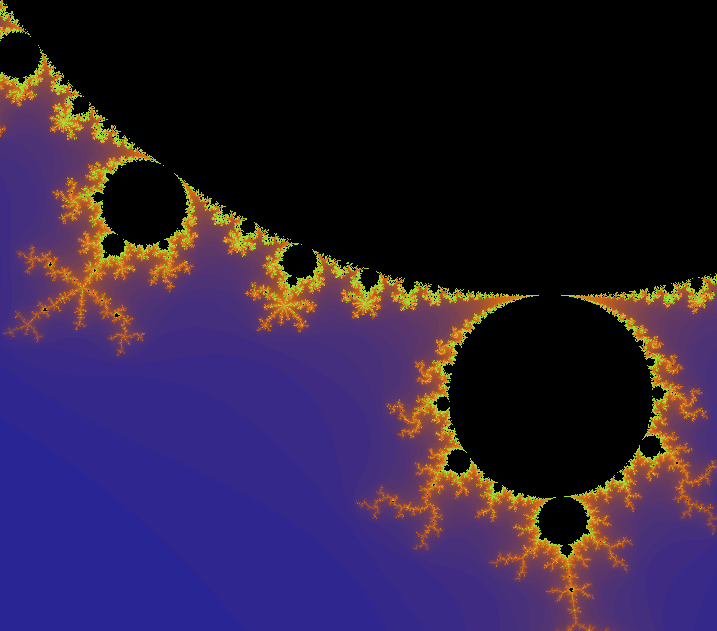
\includegraphics[scale=0.255]{./img/C3/detalle-Mandelbrot.png} \\
  (a) Conjunto completo & (b) Detalle ampliado  \\[6pt]
  \end{tabular}
    \caption{Primeras imágenes del conjunto de Mandelbrot}
    \label{fig:mandelbrot-intro}
\end{figure}

En este capítulo aprenderemos qué elementos componen estos conjuntos, y cómo llegar a estas imágenes tan llamativas.

\section{Iteración convergente y no convergente}

Recordamos que en el capítulo \refname{chap:iteracion}, a partir de una función analítica $f:\C\longrightarrow\C$, se le aplicaba una transformación $N_f(z)$ de forma que en muchos casos la iteración de dicha función era convergente independientemente del término $z_0\in\C$ inicial. Sin embargo recordemos que la iteración de una función cualquiera $f$ no siempre es convergente, como pudimos comprobar en el ejemplo situado al comienzo de la sección \ref{subsection:convergencia-punto-fijo}, en el que comprobamos que las iteradas de la función $f(z)=z^2$ divergen siempre que $|z_0|>1$, convergen a $0$ si $|z_0|<1$ y quedan encerradas en $S^1$ en caso de que $|z_0|=1$. Otro posible comportamiento es el cíclico, como el que tienen las iteradas de la función $g(z)=z\cdot i$ en $z_0=1$, que si nos fijamos, $O_g(1)=\{1,i,-1,-i,1,\dots\}$. 

Un último caso de posible comportamiento de una órbita son las órbitas caóticas, en las cuales no se percibe ningún patrón y además es muy sensible a las condiciones iniciales, fijémonos en lo que ocurre en el caso de la función $h(z)=z^2-1.9$ si miramos sus órbitas en $z_0=0,0.1$:

\begin{verbatim}
In[]:= h[z_] := z^2 - 1.9;
    NestList[h, 0.1, 20]
    NestList[h, 0.0, 20]


Out[]= {0.1, -1.89, 1.6721, 0.895918, -1.09733, -0.695866,
    -1.41577, 0.104404, -1.8891, 1.6687, 0.884552, -1.11757, 
    -0.651043, -1.47614, 0.279, -1.82216, 1.42026, 0.117148, 
    -1.88628, 1.65804, 0.849092}

Out[]= {0., -1.9, 1.71, 1.0241, -0.851219, -1.17543, -0.518374, 
  -1.63129, 0.761102, -1.32072, -0.155688, -1.87576, 1.61848, 
  0.719477, -1.38235, 0.0109007, -1.89988, 1.70955, 1.02256, 
  -0.854379, -1.17004}
\end{verbatim}

No se observa ningún patrón de convergencia y además, a pesar de ser semillas muy cercanas, las órbitas son muy diferentes.

La dicotomía existente entre qué $z_0$ iniciales hacen que las iteradas de una función coverga o no, restringida a cierta familia de funciones es la que define a los distintos conjuntos de Julia. Presentamos por tanto, para cada $c\in\C$, la familia de funciones
\begin{equation}
  P_c(z) = z^2 +c \ \ \forall z\in\C
\end{equation}

Nuestro objetivo es entonces clasificar para qué $z_0\in\C$, las iteradas $\{P_c^n(z_0)\}$ convergen, divergen, ciclan, o tienen posiblemente un comportamiento caótico.

\section{Conjuntos de Julia}

Sin dejar de tener en cuenta la familia de funciones $\{P_c(z)\}_{c\in\C}$ introducimos la siguiente definición.

\begin{definicion}
  Dado un número complejo $c\in\C$ fijo consideramos $P_c(z)=z^2+c$. Entonces:
  \begin{itemize}
    \item Se denomina \textbf{conjunto de puntos de escape}, y denotamos como $\mathsf{E}_c$ al conjunto de puntos cuyas iteradas divergen, es decir:
    $$
    \mathsf{E}_c = \{z_0\in\C: \{|P_c^n(z_0)|\}\rightarrow \infty \}
    $$
    \item  Se denomina \textbf{conjunto de puntos prisioneros}, y denotamos como $\mathsf{P}_c$ al conjunto de puntos cuyas iteradas no divergen, por lo que es el complemento de $\mathsf{E}_c$.
  \end{itemize}
\end{definicion}

A partir de estas dos definiciones, que insisten en clasificar los puntos del plano complejo entre de escape o prisioneros según su órbita, podemos introducir la definición que esperábamos.

\textit{Y aquí profesor tengo una duda porque las órbitas con comportamiento caótico, ¿se considera que divergen o no? Porque teóricamente es impredicible, pero por otro lado, en el libro pone que en la frontera entre estos dos conjuntos, es decir, en el conjunto de Julia, es donde este comportamiento es caótico, estando los detalles en cierto libro que puedo buscar, ¿lo busco o lo dejo así superficial?}

\begin{definicion}[Conjunto de Julia]
Dado un número $c\in\C$, se define su \textbf{conjunto de Julia}, y se denota como $\mathsf{J}_c$ a la frontera de $\mathsf{E}_c$.  
\end{definicion}

\begin{ejemplo}
  En el caso $c=0$, es decir, $P_0(z)=z^2$, sabemos ya que $E_c=S^1$, pues precisamente es $S^1$ la frontera entre los puntos cuyas iteradas divergen o convergen a $0$.
\end{ejemplo}

\begin{observacion}
  Fijémonos por tanto que hay tantos conjuntos de Julia como números complejos, al poder asociar a cada número complejo un conjunto de puntos prisioneros, de escape, y por tanto un conjunto de Julia.
\end{observacion}

\subsection{Representación gráfica de los conjuntos de Julia}

Tenemos entonces una definición de los conjuntos de Julia, pero aparentemente está muy alejada de las imágenes \ref{fig:julia-intro} que presentamos en la introducción. La forma de llegar a ellas es similar a la que utilizamos para graficar las imágenes que utilizaban la velocidad de convergencia en el capítulo \ref{chap:iteracion}. Sin embargo, y al contrario que al utilizar el método de Newton, ahora no tenemos ningún tipo de convergencia asegurada, por lo que el método de aplicar iteradas hasta encontrar un patrón no es el más correcto.